\documentclass[aspectratio=169]{beamer}
\usepackage{basileabeam}
\usepackage[ruled,vlined]{algorithm2e}
\usepackage{algorithmic}
\usepackage{multicol}
\usepackage{tabularray}
\usepackage[english]{babel}
\usepackage{graphicx}
\usepackage{tikz}
\graphicspath{ {./images/} }
% for inline command formatting
\definecolor{codeColor}{gray}{0.85}
\usepackage{tcolorbox}
\newtcbox{\ilc}{on line, boxrule=0pt, boxsep=0pt, bottom = 2pt, left=2pt, right =2pt, top = 2pt, arc = 0pt, colback=codeColor, colframe = white, fontupper={\small \ttfamily}}

% Notes:
%\pgfpagesuselayout{2 on 1}[a4paper,border shrink=5mm]
%\setbeamertemplate{note page}[plain]
%\setbeameroption{show notes on second screen=bottom}

\title              {Managing Resources of Network Nodes Using Append-Only-Logs}

\author             {Simon Laube, simon.laube@stud.unibas.ch}

\institute          {Advisor: Prof. Dr. Christian Tschudin, 
                    Supervisor: Fabrizio Parrillo}

\date               {July 12, 2022}

\ulogo        		{Template/header}
\ulistelement    	{Template/listelement}

\graphicspath{{./images/}}

% Options:
\totalNoSlidesDisabled % To turn off the total number of slides in the footer. Comment this if you want the total number of slides in the footer
%\headerSectionsDisabled % Comment this if you want a fancy header containing your sections.


\begin{document}

\setbeamercovered{invisible}
\setbeamercovered{again covered={\opaqueness<1->{100}}}

\begin{frame}[t,plain]
\titlepage
\end{frame}

\note{Notes can help you to remember important information. Turn on the notes option.}

% ---------------------------------------------------
\section*{Content}	

\begin{frame}
\frametitle{Content} 
\tableofcontents
\end{frame}

%% to exclude slides from presentation
%\begin{frame}<presentation:0>[noframenumbering]{...}

% ----------------------------------------------------------------
\section{Motivation}

\begin{frame}[c]{Motivation}
\begin{itemize}
    \item Solar Community Network
\end{itemize}        
\end{frame}

% ----------------------------------------------------------------
\section{Goals}

\begin{frame}[c]{Initial Goals}
\begin{itemize}
    \item Affordable Hardware
    \item Long Transmission Range (Wireless)
    \item Resilient Communication Protocol
    \begin{itemize}
    	\item Low Power Consumption
    	\item Low Storage Usage
    \end{itemize}
    \item Hardware + Software $\rightarrow$ Proof-of-Concept
    
\end{itemize}        
\end{frame}

\begin{frame}[c]{Thesis Focus}
\begin{itemize}
    \item Affordable Hardware
    \item Long Transmission Range (Wireless)
    \item \textbf{Resilient Communication Protocol}
    \begin{itemize}
    	\item \textbf{Low Power Consumption}
    	\item \textbf{Low Storage Usage}
    \end{itemize}
    \item \textbf{Hardware + Software $\rightarrow$ Proof-of-Concept}
\end{itemize}        
\end{frame}

\begin{frame}[c]{Resilient Communication Protocol}
\begin{itemize}
    \item TinySSB
    	\begin{itemize}
	    \item Tiny Version of Secure Scuttlebutt (Peer-to-Peer Communication Protocol) 
    	    \item Append-Only-Logs
    	    \item Trust Anchors and Chain of Trust
	\end{itemize}
\end{itemize}        
\end{frame}

% ----------------------------------------------------------------
\section{TinySSB}

\begin{frame}[c]{Feeds}
\begin{itemize}
    \item Everything Stored in Feeds
    \item Child Feeds
    \item Continuation Feeds
\end{itemize}        
\end{frame}

\begin{frame}[c]{Limitation: Reverting Packets}
\begin{itemize}
\end{itemize}        
\end{frame}

\begin{frame}[c]{Addition: Fork-Tree}
\begin{itemize}
    \item ...
\end{itemize}        
\end{frame}

\begin{frame}[c]{Limitation: Deleting Old Packets}
\begin{itemize}
\end{itemize}        
\end{frame}

\begin{frame}[c]{Addition: Session-Tree}
\begin{itemize}
    \item ...
\end{itemize}        
\end{frame}

% ----------------------------------------------------------------
\section{Development Process}

\begin{frame}[c]{Development Setup}
\begin{itemize}
    \item Micropython
    \item Test Code on Computer (use UDP)
    \item Test Code on LoPy 4 (use LoRa)
\end{itemize}        
\end{frame}

\begin{frame}[c]{Issues}
\begin{itemize}
    \item Stack Overflows
    	\begin{itemize}
	    \item Too much memory usage (not noticed on computer)
	    \item Format of LoPy 4 disk
	\end{itemize}
    \item Testing on LoPy much slower (e.g. Ed25519)
    \item PyMakr Extension (Visual Studio, Atom)
\end{itemize}        
\end{frame}

\begin{frame}[c]{Issues}
    \begin{figure}
        \begin{columns}[onlytextwidth]
            \column{.78\linewidth}
            \begin{onlyenv}<1>%
            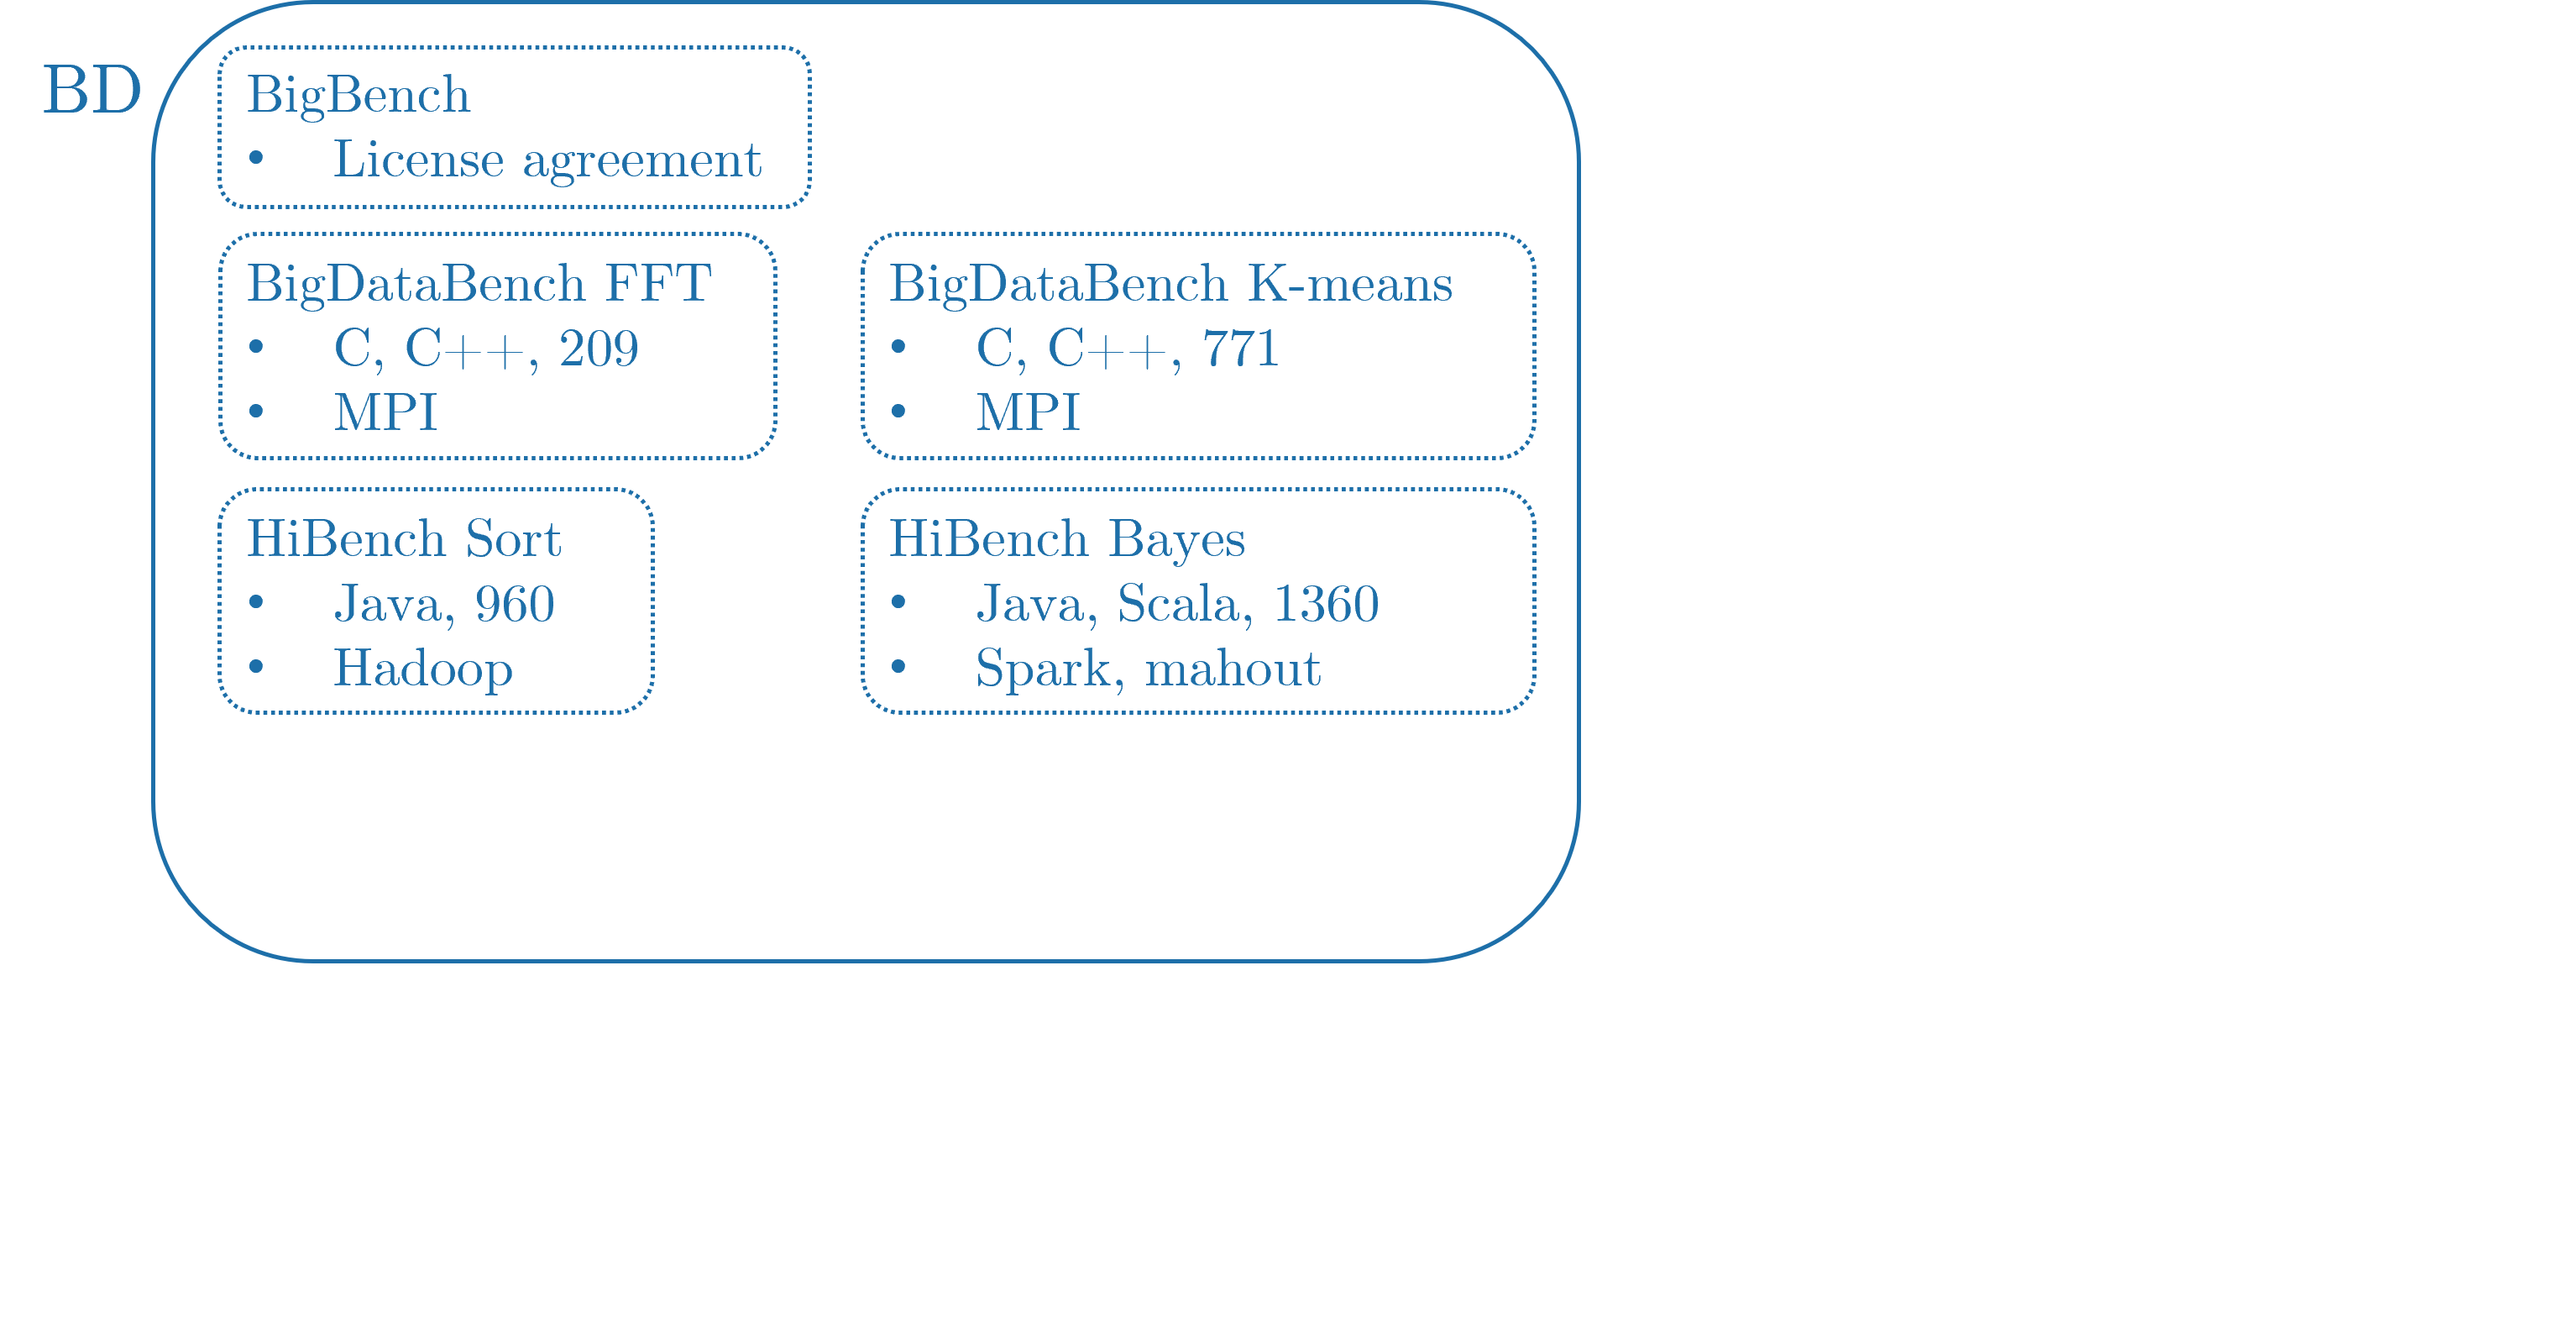
\includegraphics[width=1\textwidth]{images/Benchmarks_BD.png}%
            \end{onlyenv}
            \begin{onlyenv}<2>%
            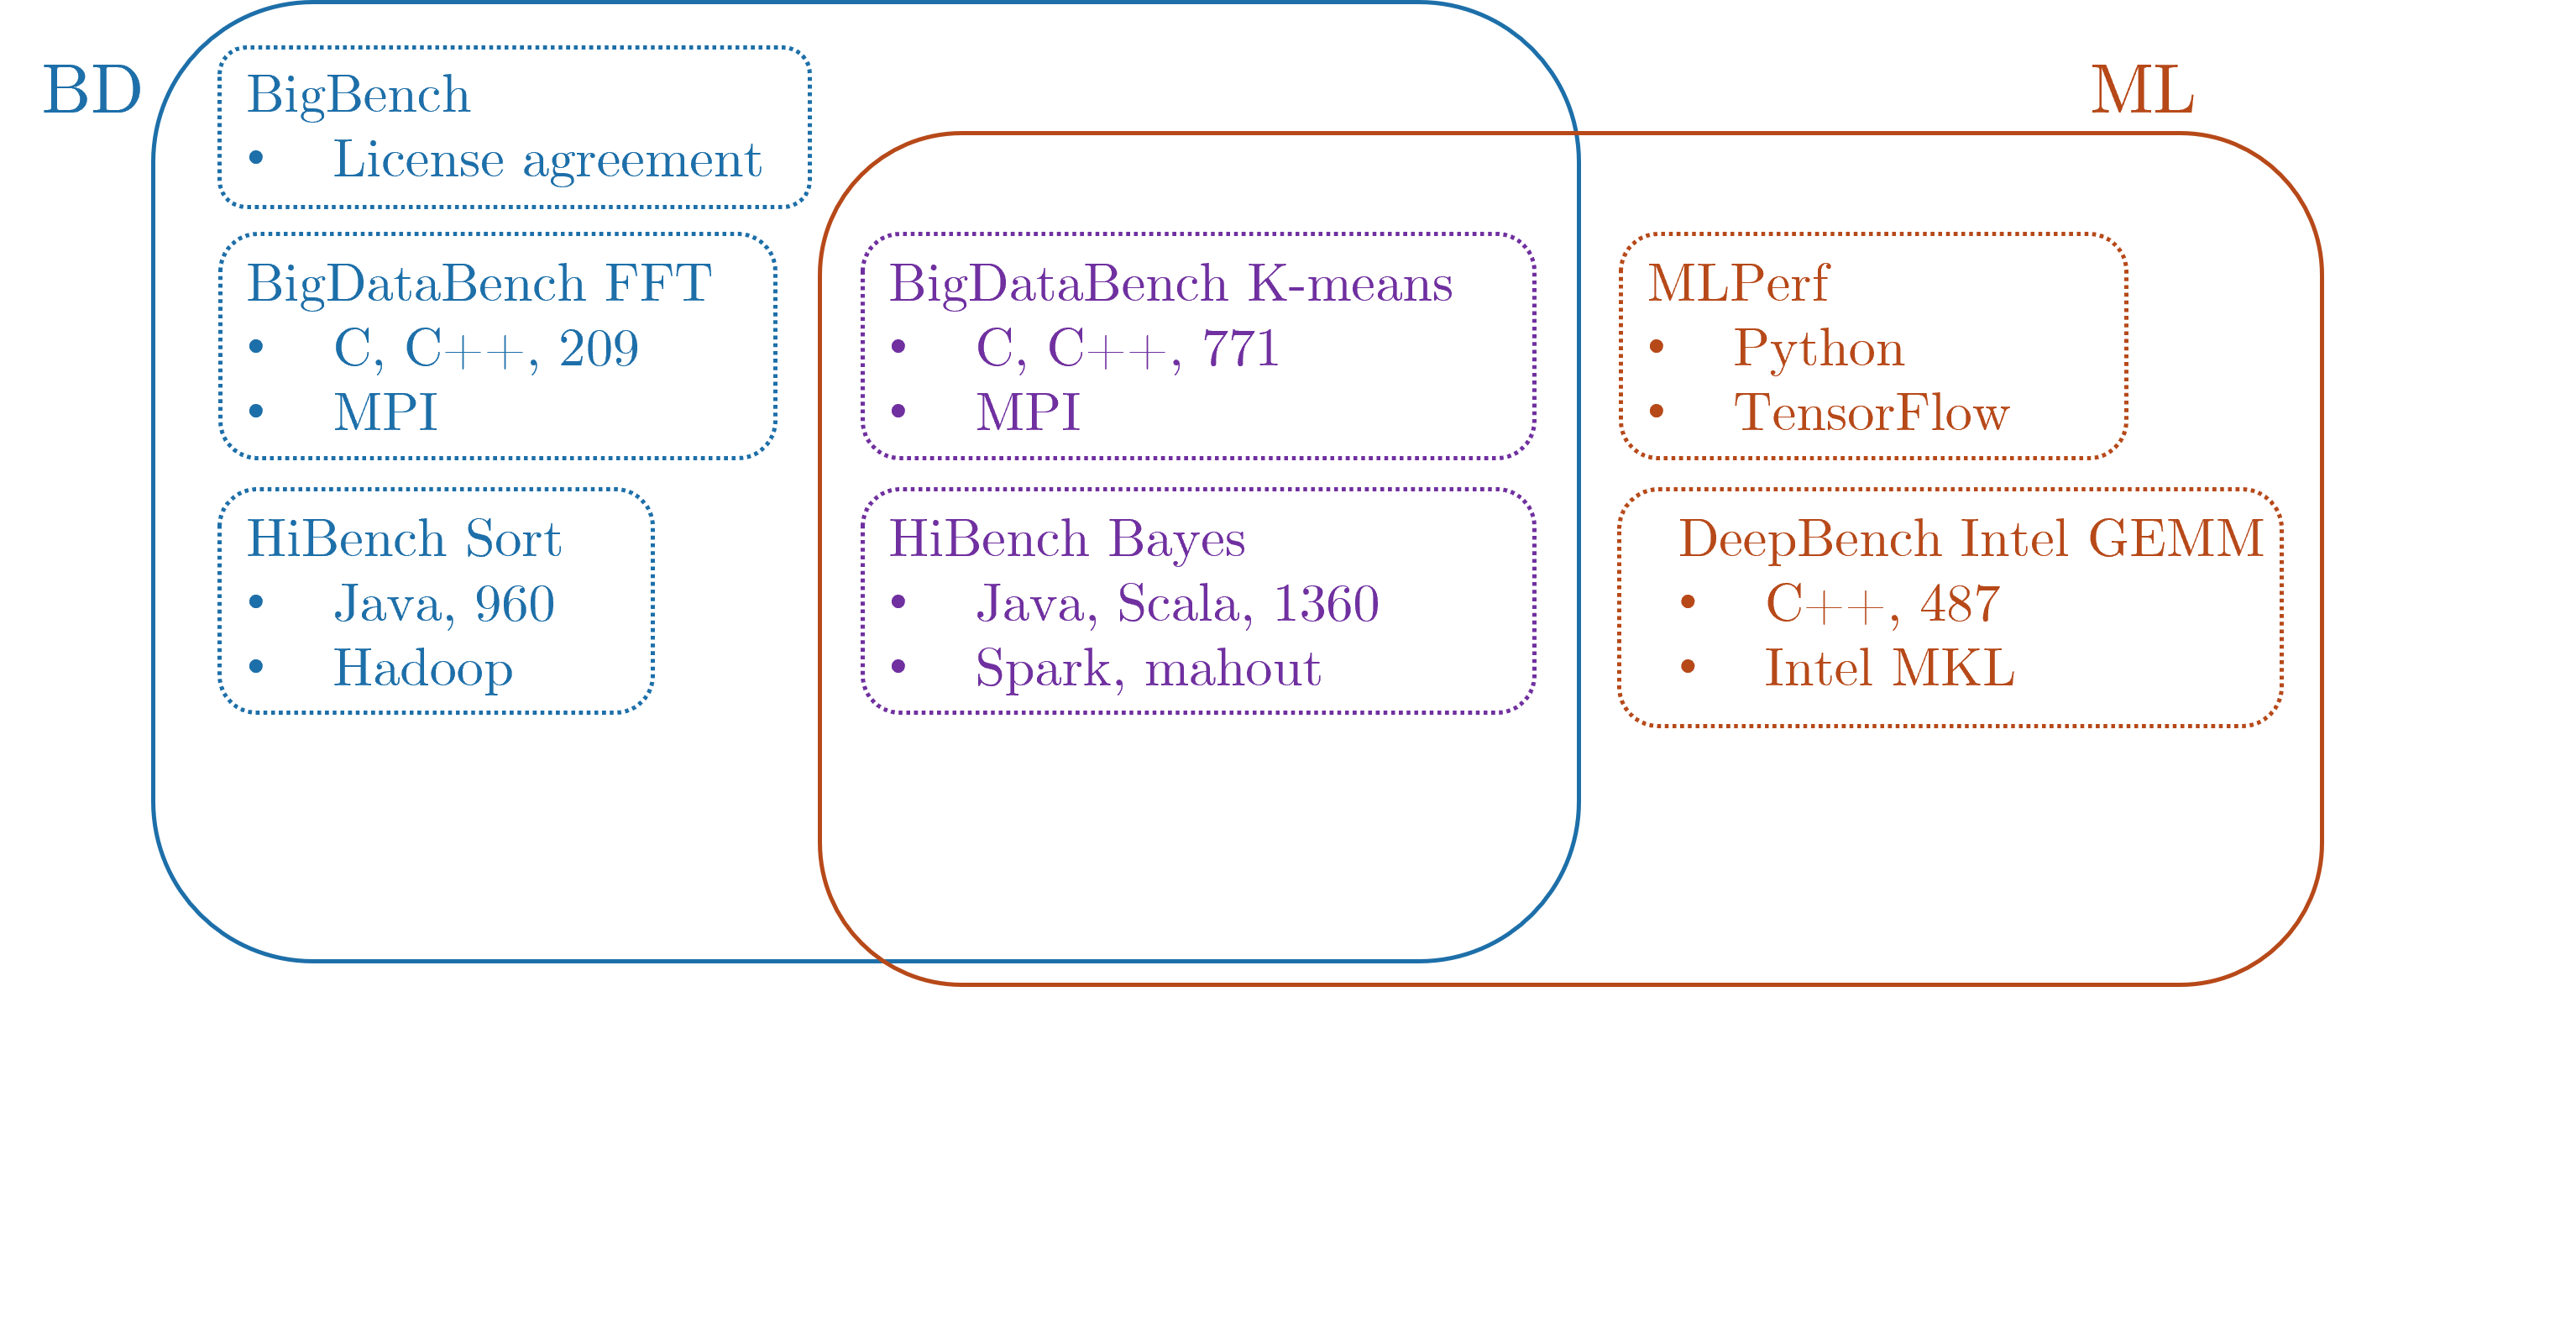
\includegraphics[width=1\textwidth]{images/Benchmarks_BDML.png}%
            \end{onlyenv}
            \begin{onlyenv}<3>%
            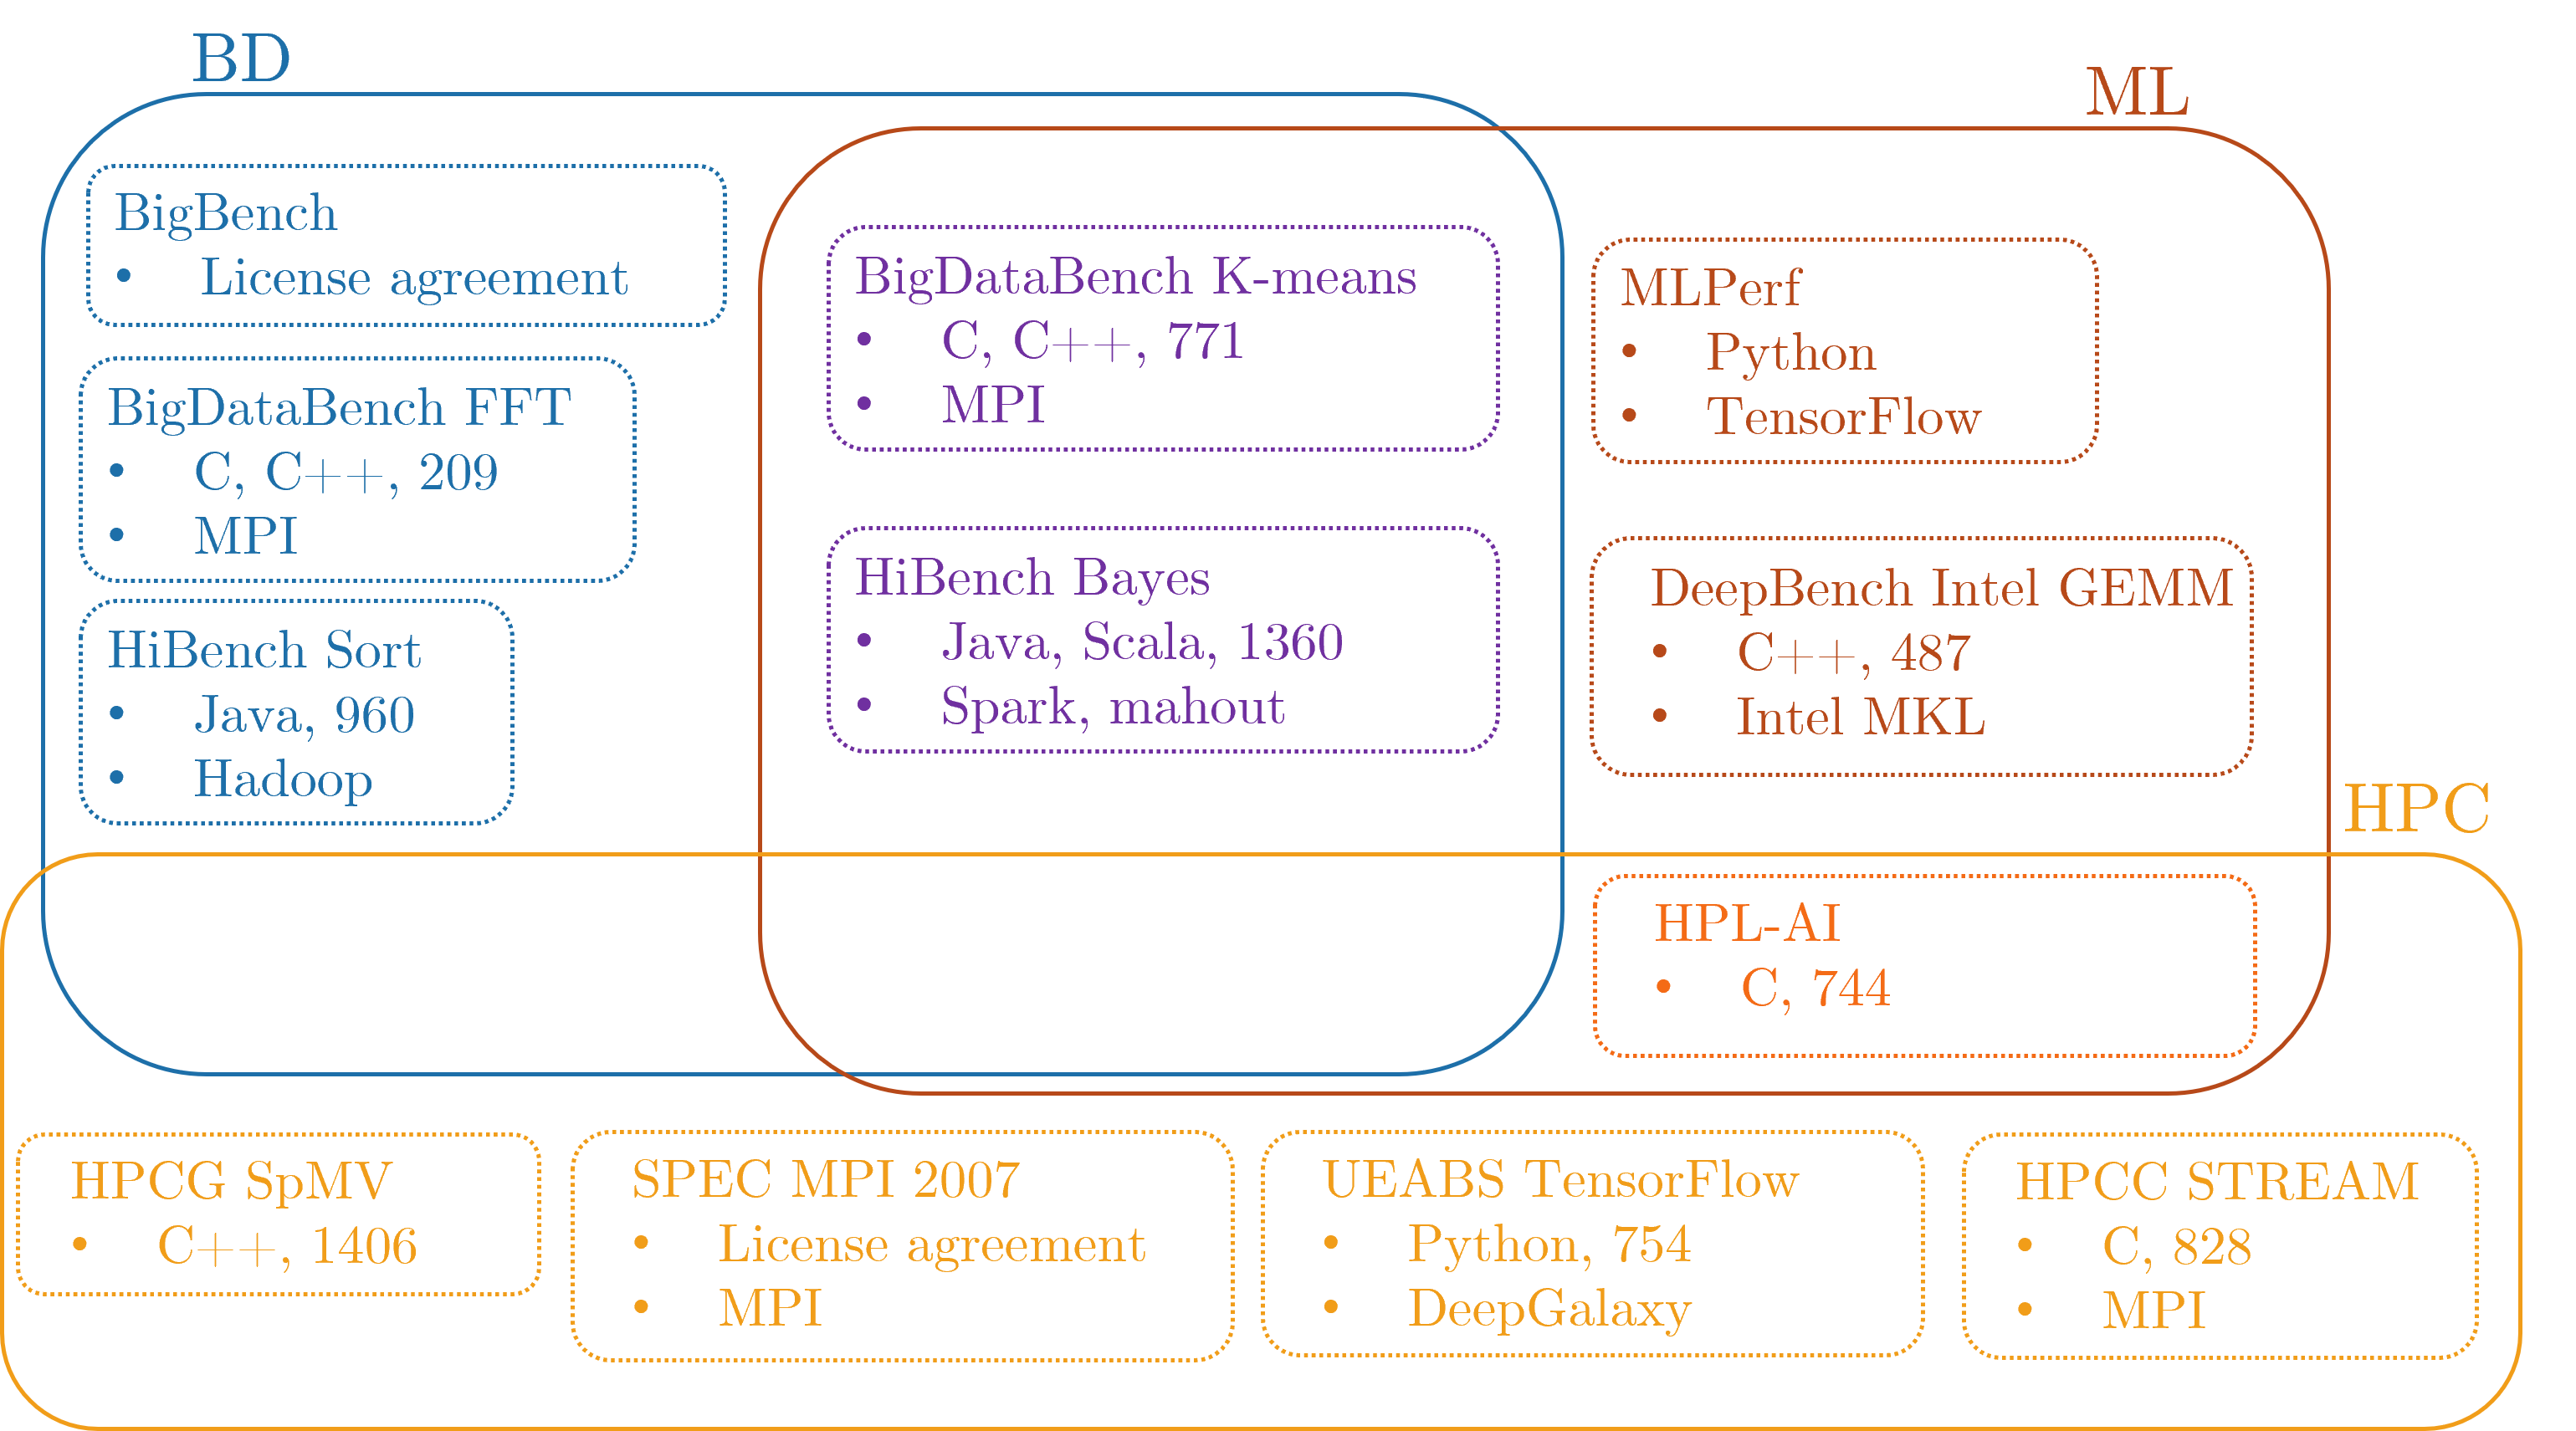
\includegraphics[width=1\textwidth]{images/Benchmarks_ALL.png}%
            \end{onlyenv}    
            \begin{onlyenv}<4>%
            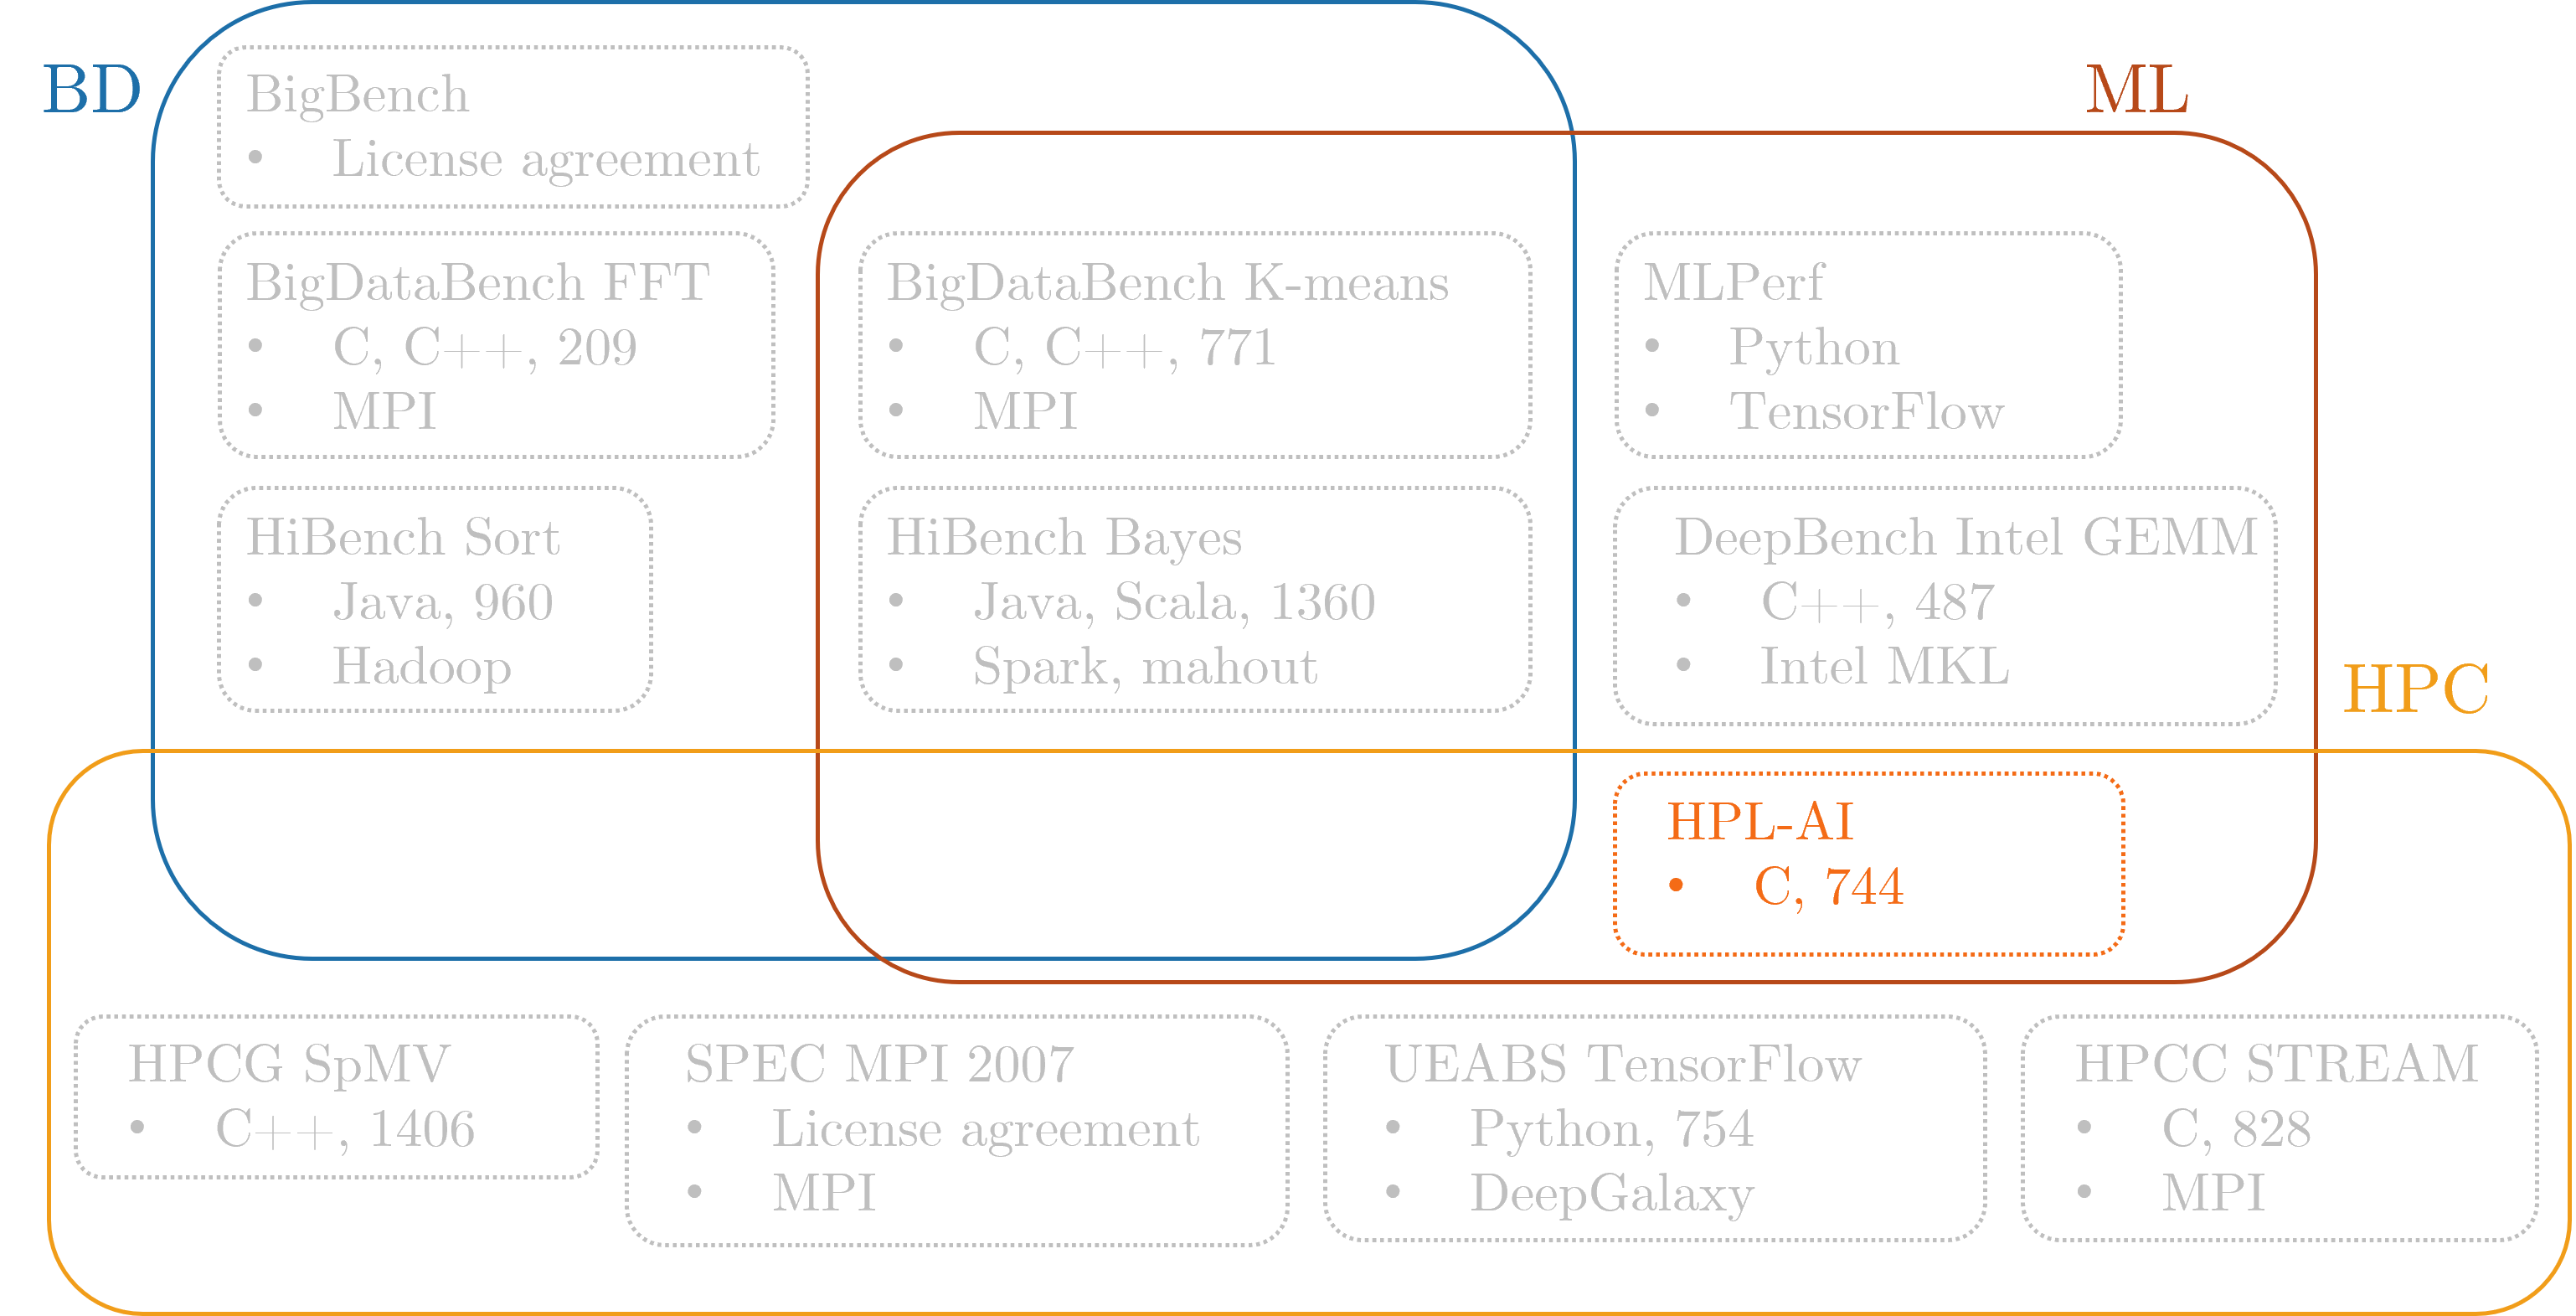
\includegraphics[width=1\textwidth]{images/Benchmarks_SEL.png}%
            \end{onlyenv}              
            \column{.2\linewidth}
            \begin{itemize}
                \item Domain
                \item Benchmark
                \item Language
                \item LOC
                \item third-party software
            \end{itemize}
        \end{columns}        
    \end{figure}          
\end{frame}


% ----------------------------------------------------------------
\section{Implementation}

\begin{frame}[c]{HPL-AI}
\begin{itemize}
    \item Solving a linear system $Ax=b$ with LU decomposition.
    \item Generating random $A$ and $b$ double precision.
    \item Convert $A$ and $b$ to single precision.
    \item Decompose $A=LU$. Solve $Ly=b$ forwards and $Ux=y$ backwards.
    \item Convert $x$ back to double precision and reinstate accuracy with generalized minimal residual method (GMRES).
\end{itemize}   
\end{frame}

\begin{frame}[c]{Code snippets}
    \begin{figure}
        \begin{columns}[onlytextwidth,t]
            \column{.5\linewidth}
            Implemented function to convert matrix from double to single precision: \\
            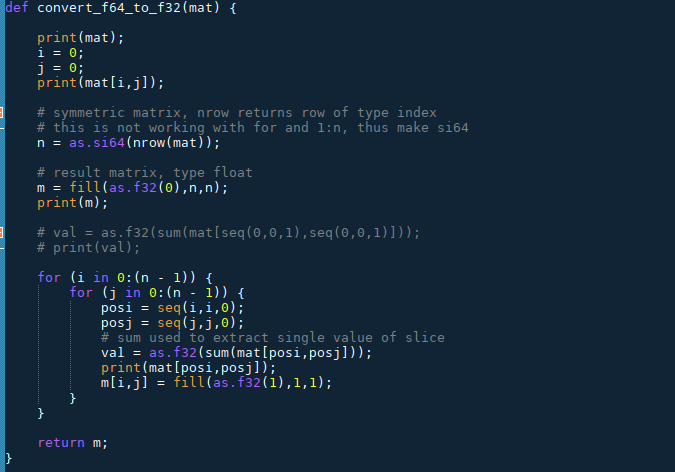
\includegraphics[width=0.9\textwidth]{images/HPL_AI_convertTof32.png}
            \column{.5\linewidth}
            Implemented function for LU decomposition: \\
            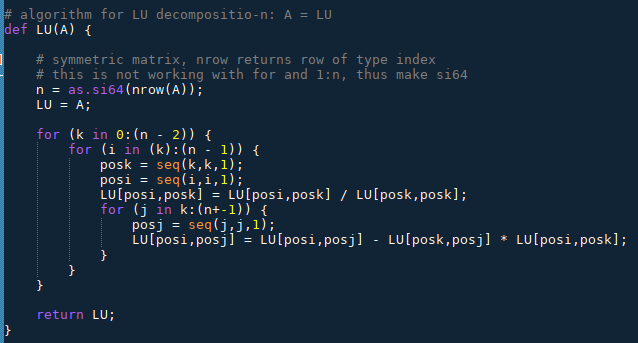
\includegraphics[width=0.9\textwidth]{images/HPL_AI_LU.png}
        \end{columns}        
    \end{figure}          
\end{frame}

\begin{frame}{Reported DaphneDSL issues}
\begin{table}[hb!]
\tiny
    \centering
    \begin{tblr}{width=0.95\textwidth, colspec={Q[c,m,wd=10mm]|Q[l,m,wd=35mm]|Q[l,m,wd=60mm]|Q[l,m]},stretch=1.1} 
        GitHub &  Issue & Description & Type   \\ 
        \hline\hline
        \href{https://github.com/daphne-eu/daphne/issues/350}{\#350} & Rbind row Check & rbind() checking number of rows instead of columns & Bug \\
        \hline              
        ? & Parsing $n-1$ & Parsing only works if there is a space after the $-$, i.e. $n-$ $1$ &  Bug\\
        \hline              
        \href{https://github.com/daphne-eu/daphne/issues/351}{\#351} & Printing with variables & Printing with calculated variables behaving differently than with assigned variables &  Bug\\
        \hline     
        \href{https://github.com/daphne-eu/daphne/issues/352}{\#352} & Integer matrix multiplication & Integer vector multiplication not working & Bug\\
        \hline       
        \href{https://github.com/daphne-eu/daphne/issues/353}{\#353} & Right indexing in loops & Right indexing with variables in loops is different from outside and is not working in functions &  Bug\\
        \hline       
        \href{https://github.com/daphne-eu/daphne/issues/354}{\#354} & Left indexing in loops & Left indexing with variables in loops is different from outside and is not working in functions &  Bug\\
        \hline       
        \href{https://github.com/daphne-eu/daphne/issues/355}{\#355} & Return from nrow() & retrun value from nrow() not usable in operation  & Bug \\ 
        \hline       
        \href{https://github.com/daphne-eu/daphne/issues/356}{\#356} & Type casting matrix & Casting on matrices not working &  Bug \\  
        \hline       
        \href{https://github.com/daphne-eu/daphne/issues/357}{\#357} & typeof() function & function returning the type of an object  & Nice to have \\    
        \hline       
        \href{https://github.com/daphne-eu/daphne/issues/358}{\#358} & Matrix literals & Simple way to create a not random value matrix & Nice to have \\       
        \hline\hline        
    \end{tblr}
\end{table} 
\end{frame}

\begin{frame}[c]{Code for issues: Bugs}
    \begin{figure}
        \begin{columns}[onlytextwidth,t]
            \column{.5\linewidth}
            Rbind row check: \\
            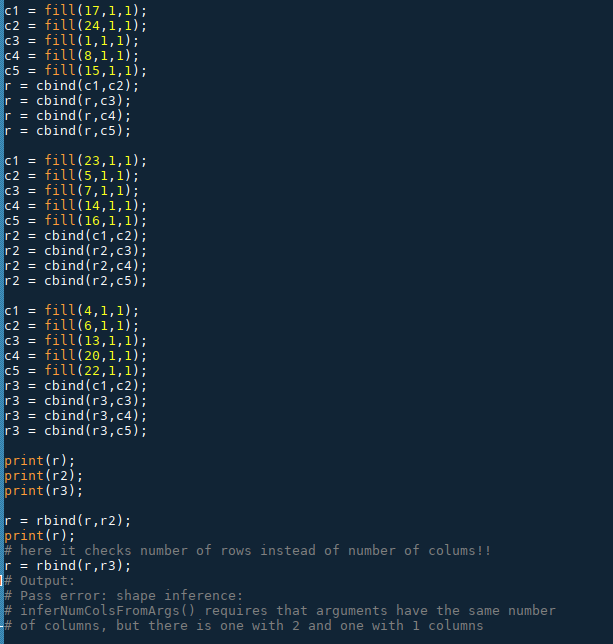
\includegraphics[width=0.8\textwidth]{images/I1.png}
            \column{.5\linewidth}
            Parsing $n-1$: \\
            
\includegraphics[width=0.9\textwidth]{images/I2.png}
        \end{columns}        
    \end{figure}          
\end{frame}

\begin{frame}[c]{Code for issues: Bugs}
    \begin{figure}
        \begin{columns}[onlytextwidth,t]
            \column{.5\linewidth}
            Printing with variables: \\
            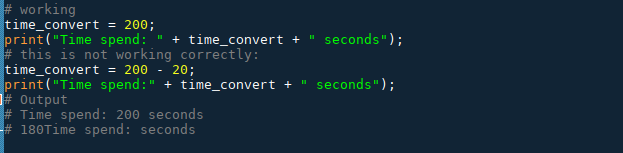
\includegraphics[width=0.9\textwidth]{images/I3.png}
            \column{.5\linewidth}
            Integer matrix multiplication: \\
            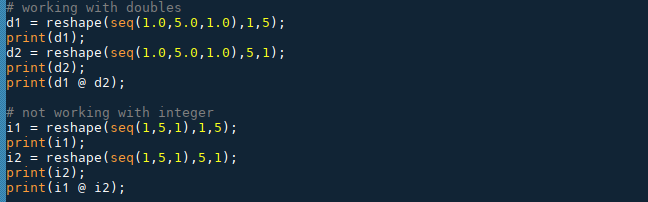
\includegraphics[width=0.9\textwidth]{images/I4.png}
        \end{columns}        
    \end{figure}          
\end{frame}

\begin{frame}[c]{Code for issues: Bugs}
    \begin{figure}
        \begin{columns}[onlytextwidth,t]
            \column{.5\linewidth}
            Right indexing in loops: \\
            
\includegraphics[width=0.9\textwidth]{images/I5.png}
            \column{.5\linewidth}
            Left indexing in loops: \\
            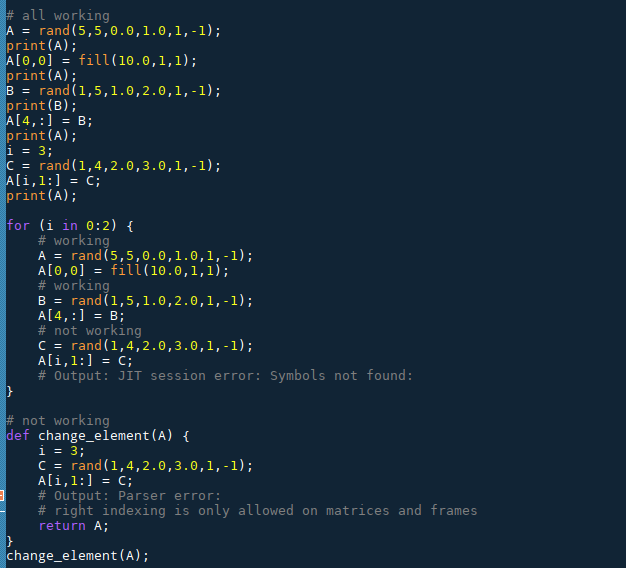
\includegraphics[width=0.9\textwidth]{images/I6.png}
        \end{columns}        
    \end{figure}          
\end{frame}

\begin{frame}[c]{Code for issues: Bugs}
    \begin{figure}
        \begin{columns}[onlytextwidth,t]
            \column{.5\linewidth}
            Return from nrow(): \\
            
\includegraphics[width=0.9\textwidth]{images/I7.png}
            \column{.5\linewidth}
            Type casting matrix: \\
            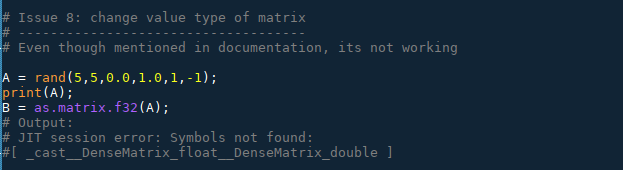
\includegraphics[width=0.9\textwidth]{images/I8.png}
        \end{columns}        
    \end{figure}          
\end{frame}

\begin{frame}[c]{Code for issues: Nice to have}
    \begin{figure}
        \begin{columns}[onlytextwidth,t]
            \column{.5\linewidth}
            typeof() function: \\
            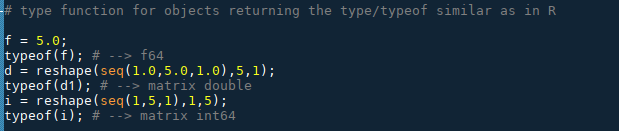
\includegraphics[width=0.9\textwidth]{images/I101.png}
            \column{.5\linewidth}
            Matrix literals: \\
            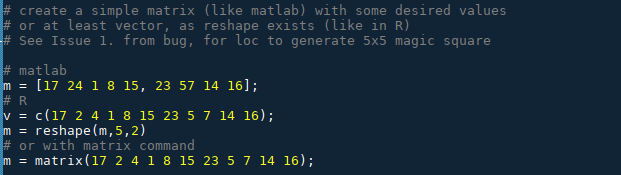
\includegraphics[width=0.9\textwidth]{images/I102.png}
        \end{columns}        
    \end{figure}          
\end{frame}

\begin{frame}{Another way: Using built in functionality}
\begin{itemize}[<+>]
    \item Using DaphneDSL \ilc{as.} for casting and \ilc{solve} to solve linear system.
    \item Advantage: Few lines of code if available.
    \item Disadvantage: \ilc{solve} is not vectorized.
    \item Disadvantage: Not knowing what is actually happening inside DAPHNE
\end{itemize}     
\end{frame}


% ----------------------------------------------------------------
\section{Next steps and challenges}

\begin{frame}{Next steps}
\begin{itemize}
    \item Find benchmarks implementable given the current state of DaphneDSL.
    \item Open new issues on GitHub for additional problems.
\end{itemize}     
\end{frame}

\begin{frame}{Challenges}
\begin{itemize}[<+>]
    \item The timeline of the thesis is not matching the time horizon for solving issues
    \item DAPHNE is an ongoing project and things are not finished yet (e.g. documentation)
    \item Any questions or suggestions?
\end{itemize}     
\end{frame}


% dont use that in HPC group
\begin{frame}<presentation:0>[t,plain]
\lastpage{{\usebeamerfont{title}Questions? Suggestions? Ideas?}\\[5ex]
reto.krummenacher@unibas.ch}
\end{frame}

\end{document}
